\documentclass{standalone}
\usepackage{tikz}
\usetikzlibrary{patterns, positioning}
\usepackage[sfdefault]{ClearSans} %% option 'sfdefault' activates Clear Sans as the default text font
\usepackage[T1]{fontenc}

\begin{document}
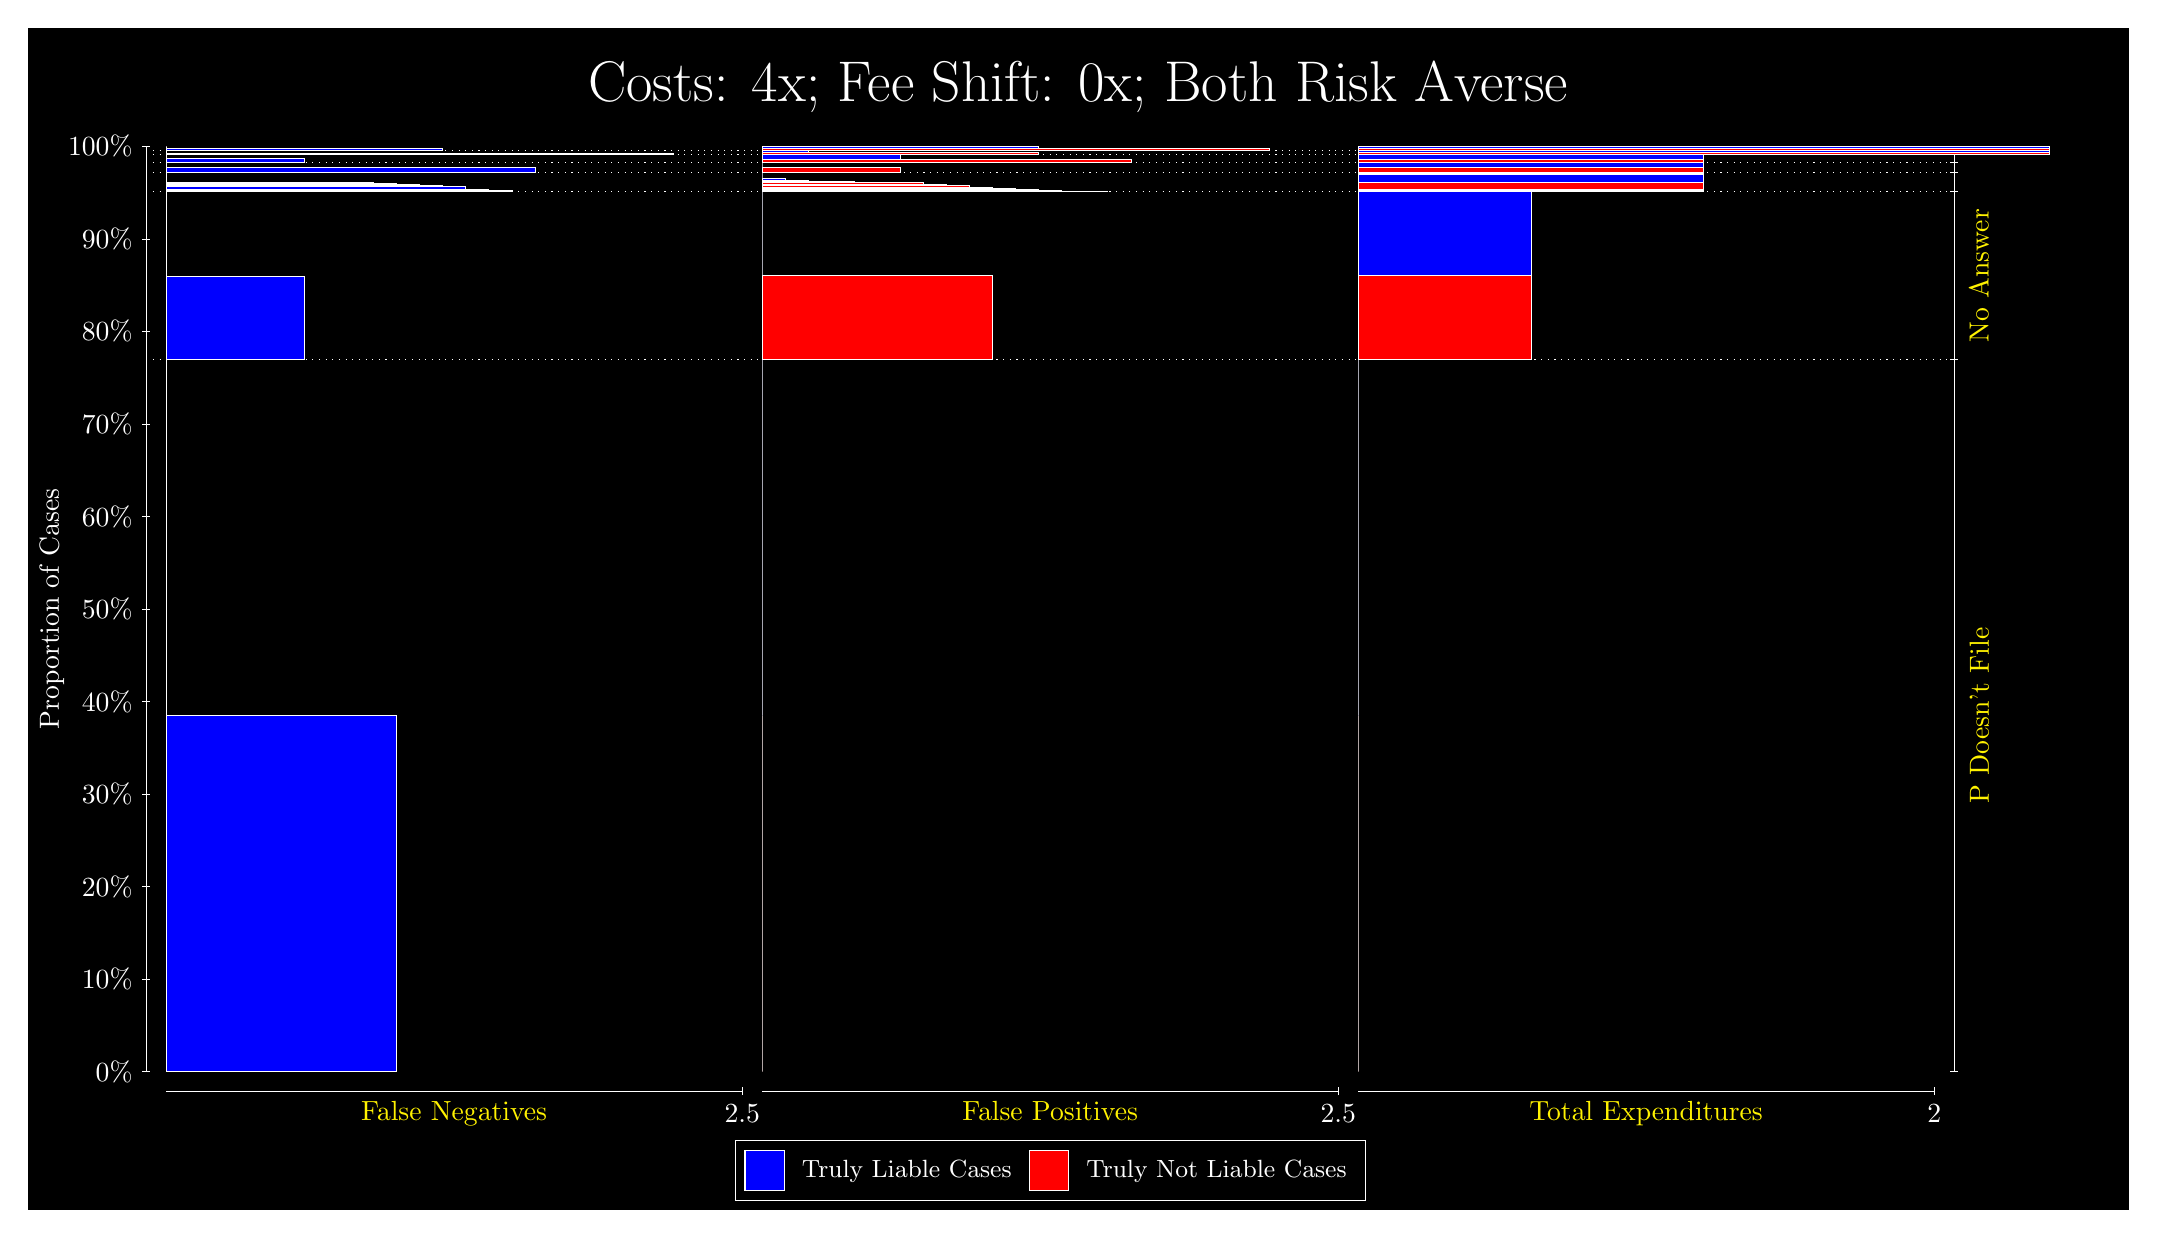
\begin{tikzpicture}
\draw[fill=black] (0,0) rectangle (26.667,15);
\draw[text=white] (0,13.5) rectangle (26.667,15) node[midway] {\huge Costs: 4x; Fee Shift: 0x; Both Risk Averse};
\draw[white, very thin] (1.5,1.75) -- (1.5,13.5);
\node[rotate=90, text=white, anchor=center] at (0.3, 7.625) {Proportion of Cases};
\draw[white, very thin] (1.45,1.75) -- (1.55,1.75);
\node[text=white, anchor=east] at (1.45, 1.75) {0\%};
\draw[white, very thin] (1.45,2.925) -- (1.55,2.925);
\node[text=white, anchor=east] at (1.45, 2.925) {10\%};
\draw[white, very thin] (1.45,4.1) -- (1.55,4.1);
\node[text=white, anchor=east] at (1.45, 4.1) {20\%};
\draw[white, very thin] (1.45,5.275) -- (1.55,5.275);
\node[text=white, anchor=east] at (1.45, 5.275) {30\%};
\draw[white, very thin] (1.45,6.45) -- (1.55,6.45);
\node[text=white, anchor=east] at (1.45, 6.45) {40\%};
\draw[white, very thin] (1.45,7.625) -- (1.55,7.625);
\node[text=white, anchor=east] at (1.45, 7.625) {50\%};
\draw[white, very thin] (1.45,8.8) -- (1.55,8.8);
\node[text=white, anchor=east] at (1.45, 8.8) {60\%};
\draw[white, very thin] (1.45,9.975) -- (1.55,9.975);
\node[text=white, anchor=east] at (1.45, 9.975) {70\%};
\draw[white, very thin] (1.45,11.15) -- (1.55,11.15);
\node[text=white, anchor=east] at (1.45, 11.15) {80\%};
\draw[white, very thin] (1.45,12.325) -- (1.55,12.325);
\node[text=white, anchor=east] at (1.45, 12.325) {90\%};
\draw[white, very thin] (1.45,13.5) -- (1.55,13.5);
\node[text=white, anchor=east] at (1.45, 13.5) {100\%};

\draw[white, very thin] (24.457,1.75) -- (24.457,13.5);
\draw[white, very thin] (24.407,1.75) -- (24.507,1.75);
\node[anchor=west] at (24.407, 1.75) {};
\draw[white, very thin] (24.407,10.792) -- (24.507,10.792);
\node[anchor=west] at (24.407, 10.792) {};
\draw[white, very thin] (24.407,12.923) -- (24.507,12.923);
\node[anchor=west] at (24.407, 12.923) {};
\draw[white, very thin] (24.407,13.168) -- (24.507,13.168);
\node[anchor=west] at (24.407, 13.168) {};
\draw[white, very thin] (24.407,13.294) -- (24.507,13.294);
\node[anchor=west] at (24.407, 13.294) {};
\draw[white, very thin] (24.407,13.393) -- (24.507,13.393);
\node[anchor=west] at (24.407, 13.393) {};
\draw[white, very thin] (24.407,13.447) -- (24.507,13.447);
\node[anchor=west] at (24.407, 13.447) {};
\draw[white, very thin] (24.407,13.5) -- (24.507,13.5);
\node[anchor=west] at (24.407, 13.5) {};

\draw[white, very thin, fill=blue] (1.75,1.75) rectangle (4.6775,6.271);
\draw[white, very thin, fill=red] (1.75,6.271) rectangle (1.75,10.792);
\draw[white, very thin, fill=blue] (1.75,10.792) rectangle (3.5065,11.855);
\draw[white, very thin, fill=red] (1.75,11.855) rectangle (1.75,12.923);
\draw[white, very thin, fill=blue] (1.75,12.923) rectangle (6.1413,12.943);
\draw[white, very thin, fill=blue] (1.75,12.943) rectangle (5.8486,12.96);
\draw[white, very thin, fill=blue] (1.75,12.96) rectangle (5.5558,12.989);
\draw[white, very thin, fill=blue] (1.75,12.989) rectangle (5.2631,13.001);
\draw[white, very thin, fill=blue] (1.75,13.001) rectangle (4.9703,13.019);
\draw[white, very thin, fill=blue] (1.75,13.019) rectangle (4.6775,13.031);
\draw[white, very thin, fill=blue] (1.75,13.031) rectangle (4.3848,13.041);
\draw[white, very thin, fill=blue] (1.75,13.041) rectangle (4.092,13.045);
\draw[white, very thin, fill=blue] (1.75,13.045) rectangle (3.7993,13.049);
\draw[white, very thin, fill=red] (1.75,13.049) rectangle (1.75,13.168);
\draw[white, very thin, fill=blue] (1.75,13.168) rectangle (6.4341,13.228);
\draw[white, very thin, fill=red] (1.75,13.228) rectangle (1.75,13.294);
\draw[white, very thin, fill=blue] (1.75,13.294) rectangle (3.5065,13.349);
\draw[white, very thin, fill=red] (1.75,13.349) rectangle (1.75,13.393);
\draw[white, very thin, fill=blue] (1.75,13.393) rectangle (8.1906,13.416);
\draw[white, very thin, fill=red] (1.75,13.416) rectangle (1.75,13.447);
\draw[white, very thin, fill=blue] (1.75,13.447) rectangle (5.2631,13.474);
\draw[white, very thin, fill=red] (1.75,13.474) rectangle (1.75,13.5);
\draw[white, very thin, fill=red] (9.3189,1.75) rectangle (9.3189,6.2711);
\draw[white, very thin, fill=blue] (9.3189,6.2711) rectangle (9.3189,10.792);
\draw[white, very thin, fill=red] (9.3189,10.792) rectangle (12.246,11.86);
\draw[white, very thin, fill=blue] (9.3189,11.86) rectangle (9.3189,12.923);
\draw[white, very thin, fill=red] (9.3189,12.923) rectangle (13.71,12.927);
\draw[white, very thin, fill=red] (9.3189,12.927) rectangle (13.417,12.931);
\draw[white, very thin, fill=red] (9.3189,12.931) rectangle (13.125,12.94);
\draw[white, very thin, fill=red] (9.3189,12.94) rectangle (12.832,12.951);
\draw[white, very thin, fill=red] (9.3189,12.951) rectangle (12.539,12.968);
\draw[white, very thin, fill=red] (9.3189,12.968) rectangle (12.246,12.979);
\draw[white, very thin, fill=red] (9.3189,12.979) rectangle (11.954,13.005);
\draw[white, very thin, fill=red] (9.3189,13.005) rectangle (11.661,13.019);
\draw[white, very thin, fill=red] (9.3189,13.019) rectangle (11.368,13.042);
\draw[white, very thin, fill=blue] (9.3189,13.042) rectangle (10.783,13.046);
\draw[white, very thin, fill=blue] (9.3189,13.046) rectangle (10.49,13.051);
\draw[white, very thin, fill=blue] (9.3189,13.051) rectangle (10.197,13.06);
\draw[white, very thin, fill=blue] (9.3189,13.06) rectangle (9.9044,13.072);
\draw[white, very thin, fill=blue] (9.3189,13.072) rectangle (9.6116,13.09);
\draw[white, very thin, fill=blue] (9.3189,13.09) rectangle (9.3189,13.168);
\draw[white, very thin, fill=red] (9.3189,13.168) rectangle (11.075,13.234);
\draw[white, very thin, fill=blue] (9.3189,13.234) rectangle (9.3189,13.294);
\draw[white, very thin, fill=red] (9.3189,13.294) rectangle (14.003,13.338);
\draw[white, very thin, fill=blue] (9.3189,13.338) rectangle (11.075,13.393);
\draw[white, very thin, fill=red] (9.3189,13.393) rectangle (12.832,13.424);
\draw[white, very thin, fill=blue] (9.3189,13.424) rectangle (9.9044,13.447);
\draw[white, very thin, fill=red] (9.3189,13.447) rectangle (15.759,13.473);
\draw[white, very thin, fill=blue] (9.3189,13.473) rectangle (12.832,13.5);
\draw[white, very thin, fill=red] (16.888,1.75) rectangle (16.888,6.2711);
\draw[white, very thin, fill=blue] (16.888,6.2711) rectangle (16.888,10.792);
\draw[white, very thin, fill=red] (16.888,10.792) rectangle (19.083,11.86);
\draw[white, very thin, fill=blue] (16.888,11.86) rectangle (19.083,12.923);
\draw[white, very thin, fill=red] (16.888,12.923) rectangle (21.279,12.939);
\draw[white, very thin, fill=blue] (16.888,12.939) rectangle (21.279,12.957);
\draw[white, very thin, fill=red] (16.888,12.957) rectangle (21.279,13.046);
\draw[white, very thin, fill=blue] (16.888,13.046) rectangle (21.279,13.141);
\draw[white, very thin, fill=red] (16.888,13.141) rectangle (21.279,13.154);
\draw[white, very thin, fill=blue] (16.888,13.154) rectangle (21.279,13.168);
\draw[white, very thin, fill=red] (16.888,13.168) rectangle (21.279,13.234);
\draw[white, very thin, fill=blue] (16.888,13.234) rectangle (21.279,13.294);
\draw[white, very thin, fill=red] (16.888,13.294) rectangle (21.279,13.338);
\draw[white, very thin, fill=blue] (16.888,13.338) rectangle (21.279,13.393);
\draw[white, very thin, fill=red] (16.888,13.393) rectangle (25.67,13.424);
\draw[white, very thin, fill=blue] (16.888,13.424) rectangle (25.67,13.447);
\draw[white, very thin, fill=red] (16.888,13.447) rectangle (25.67,13.473);
\draw[white, very thin, fill=blue] (16.888,13.473) rectangle (25.67,13.5);
\draw[white, dotted] (1.5,10.792) -- (24.457,10.792);
\draw[white, dotted] (1.5,12.923) -- (24.457,12.923);
\draw[white, dotted] (1.5,13.168) -- (24.457,13.168);
\draw[white, dotted] (1.5,13.294) -- (24.457,13.294);
\draw[white, dotted] (1.5,13.393) -- (24.457,13.393);
\draw[white, dotted] (1.5,13.447) -- (24.457,13.447);
\draw[white, very thin] (1.75,1.5) -- (9.0689,1.5);
\node[text=yellow, anchor=north] at (5.4094, 1.5) {False Negatives};
\draw[white, very thin] (9.0689,1.45) -- (9.0689,1.55);
\node[text=white, anchor=north] at (9.0689, 1.45) {2.5};

\draw[white, very thin] (9.3189,1.5) -- (16.638,1.5);
\node[text=yellow, anchor=north] at (12.978, 1.5) {False Positives};
\draw[white, very thin] (16.638,1.45) -- (16.638,1.55);
\node[text=white, anchor=north] at (16.638, 1.45) {2.5};

\draw[white, very thin] (16.888,1.5) -- (24.207,1.5);
\node[text=yellow, anchor=north] at (20.547, 1.5) {Total Expenditures};
\draw[white, very thin] (24.207,1.45) -- (24.207,1.55);
\node[text=white, anchor=north] at (24.207, 1.45) {2};

\node[text=yellow, centered, rotate=90] at (24.777, 6.2711) {P Doesn't File};
\node[text=yellow, centered, rotate=90] at (24.777, 11.857) {No Answer};






\draw (12.978300999999998,1.5) node[draw=none] (baseCoordinate) {};
\begin{scope}[align=center]
        \matrix[scale=0.5, draw=white, below=0.5cm of baseCoordinate, nodes={draw}, column sep=0.1cm]{
            \node[rectangle, draw, minimum width=0.5cm, minimum height=0.5cm, fill=blue] {}; &
            \node[draw=none, font=\small, text=white] (B) {Truly Liable Cases}; &
            \node[rectangle, draw, minimum width=0.5cm, minimum height=0.5cm, fill=red] {}; &
            \node[draw=none, font=\small, text=white] (B) {Truly Not Liable Cases}; \\
            };
\end{scope}

\end{tikzpicture}
\end{document}